\documentclass{homework}

\title{Homework 3}
\author{Kevin Evans}
\studentid{11571810}
\date{February 10, 2021}
\setclass{Physics}{342}
\usepackage{amssymb}
\usepackage{mathtools}

\usepackage{amsthm}
\usepackage{amsmath}
\usepackage{slashed}
\usepackage{relsize}
\usepackage{threeparttable}
\usepackage{float}
\usepackage{booktabs}
\usepackage{boldline}
\usepackage{changepage}
\usepackage{physics}
\usepackage[inter-unit-product =\cdot]{siunitx}
\usepackage{setspace}

\usepackage[makeroom]{cancel}
%\usepackage{pgfplots}

\usepackage{enumitem}
\usepackage{times}

\usepackage{calligra}
\DeclareMathAlphabet{\mathcalligra}{T1}{calligra}{m}{n}
\DeclareFontShape{T1}{calligra}{m}{n}{<->s*[2.2]callig15}{}
\newcommand{\scriptr}{\mathcalligra{r}\,}
\newcommand{\boldscriptr}{\pmb{\mathcalligra{r}}\,}
\newcommand{\emf}{\mathcal{E}}

\begin{document}
	\maketitle
	\begin{enumerate}
		\item Assuming the electric field is uniform and radially outward between the two cylinders, \begin{align*}
			E & = V / (b - a) % this is wrong
			\intertext{The magnetic field is given by Amp\`ere's law and is in the azimuthal direction as}
			B & = \frac{\mu_0 I}{2 \pi s}
			\intertext{As the two fields are perpendicular, the magnitude of the Poynting vector is}
			S & = \frac{1}{\mu_0} EB = \frac{VI}{2 \pi s (b-a)}
			\intertext{The Poynting vector is in the direction of the cable's length, so the respective $\dd{a}$ is over the annular face, $s \dd{\phi} \dd{s}$. Integrating this to find the total power,}
			P & = \int_S \frac{VI}{2 \pi s (b-a)} \dd{a} \\
				& = \frac{VI}{2 \pi (b-a)} \int_a^b \dd{s} \int_0^{2\pi} \dd{\phi} \\
			\Aboxed{ P & = \frac{VI}{(b-a)} (b - a) = VI}
		\end{align*}
	
		\item For each wire of density $\lambda$, the electric field is \begin{align*}
			\bvec{E} & = \frac{\lambda}{2 \pi \epsilon_0 s} \uvec{s}
		\end{align*}
		Taking the surface to be the $xy$ plane, the electric field along the plane is directed radially outward. Along the surface, the net electric field is \begin{align*}
			\bvec{E} & = \frac{ 2\lambda }{2 \pi \epsilon_0 s} \cos \theta \uvec{s} = \frac{\lambda}{\pi \epsilon_0 s} \left(\frac{x}{(x^2 + a^2)^{1/2}}\right) \uvec{x} \\
				& = \frac{\lambda}{\pi \epsilon_0} \left(\frac{x}{x^2 + a^2}\right) \uvec{x}
		\end{align*}
		As the electric field is only in the $x$ direction, the tensor can be simplified where only the $T_{zz}$ component remains, \begin{align*}
			T_{zz} & = \frac{\epsilon_0 {E_x}^2}{2} = \frac{\lambda^2}{2 \pi^2 \epsilon_0} \frac{x^2}{(x^2 + a^2)^2}
		\intertext{Thus, the force per unit length is}
		\bvec{f} & = \int_{-\infty}^\infty T_{zz} \dd{x} \uvec{x}\\
			& = \frac{\lambda^2}{2 \pi^2 \epsilon_0} \int_{-\infty}^\infty \frac{x^2}{(x^2 + a^2)^2} \dd{x} \uvec{x}\\
			& = \frac{\lambda^2}{4 \pi \epsilon_0 a}  \uvec{x}
		\end{align*}
	
		\item The diagram would look something like this: 
		
		% TODO: \usepackage{graphicx} required
		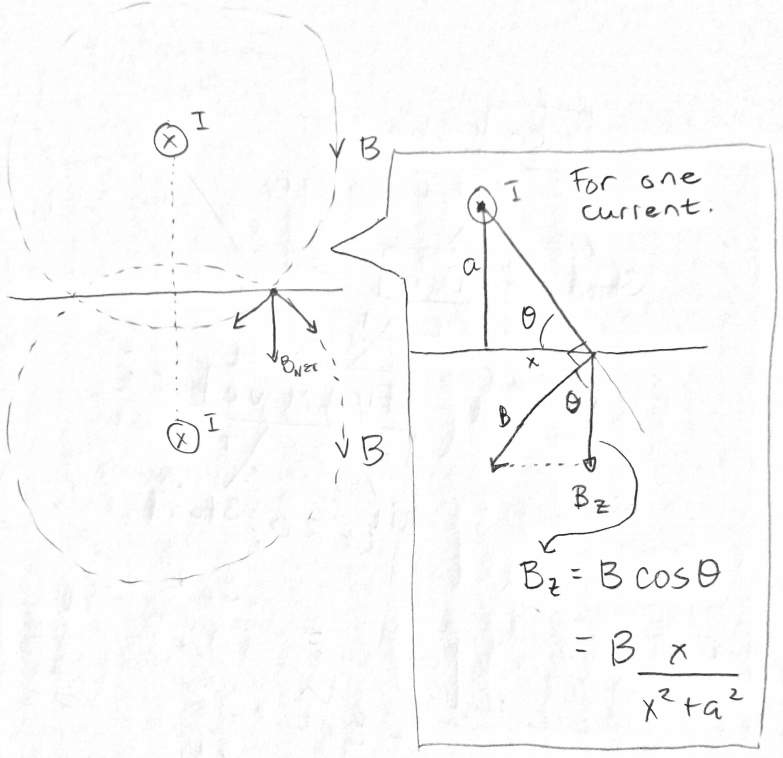
\includegraphics[width=0.7\linewidth]{hw3_diagram}
		
		From the diagram and Amp\`ere's law, the vertical component of the magnetic field for both wires is \begin{align*}
			B_z & = 2 \times \frac{\mu_0 I }{2 \pi s} \frac{x}{s} \\
				& = \frac{\mu_0 I}{\pi} \frac{x}{x^2 + a^2}
		\end{align*}
		The only non-zero component of the tensor is $T_{zz}$ acting on the $xy$ plane is \begin{align*}
			T_{zz} & = -\frac{{B_z}^2}{2 \mu_0} \\
				& = - \frac{\mu_0 I^2}{2 \pi^2} \frac{x^2}{(x^2 + a^2)^2}
		\end{align*}
		Integrating over all $x$ will give the force per unit length, \begin{align*}
			\bvec{f} & = - \frac{\mu_0 I^2}{2 \pi^2} \int_{-\infty}^\infty \frac{x^2}{(x^2 + a^2)^2} \dd{x} \uvec{z} \\
				& =  - \frac{\mu_0 I^2}{4 \pi a}
		\end{align*}
		\item For a solenoid of radius $a$, current $I$, and $n$ turns per length, within the solenoid the magnetic field is \begin{align*}
			\bvec{B} & = \mu_0 n I \uvec{z}
		\end{align*}
		And the electric field is zero as the current is assumed to be constant. So the stress tensor is \begin{align*}
			\tensor{T} & = -\frac{\mu_0 n^2 I^2}{2}  \begin{pmatrix}
				1 & 0 & 0 \\
				0 & 1 & 0 \\
				0 & 0 & 1
			\end{pmatrix}
		\end{align*}
	
		\item \begin{enumerate}
			\item Similar to Problem 1 from the last homework, the magnetic field and flux through the ring is \begin{align*}
				B & = \mu_0 n I \\
				\Phi & = \int B \dd{a} = \mu_0 n I_s \pi a^2
				\intertext{Then the emf and current is}
				\emf & = - \dot{\Phi} = -\mu_0 n \pi a^2 \dv{I_s}{t} \\
				I_r & = -\frac{\mu_0 n \pi a^2}{R} \dv{I_s}{t}
			\end{align*}
		
			\item The induced electric field due to the changing flux is \begin{align*}
				\oint \bvec{E} \cdot \dd{\bvec{l}} & = \emf\\
				E & = \emf / 2 \pi a
				\intertext{The magnetic field from $I_r$ is given by Amp\`ere's law,}
				B & = \frac{\mu_0 I_r}{2 \pi b}
				\intertext{The magnitude of the Poynting vector is}
				S & = \frac{1}{\mu_0} EB = \frac{\emf I_r}{4 \pi^2 ab}
				\intertext{Integrating over the cylindrical area of the solenoid,}
				P & = \eval{ \int_0^{2\pi} \int_0^L \frac{\emf I_r}{4 \pi ab}  s \dd{z} \dd{\phi} }_{s=a} \\
					& = \frac{\emf I_r L}{2 \pi b}
				\intertext{...not really sure where to go from here}
			\end{align*}
		\end{enumerate}
	\end{enumerate}
\end{document}